\chapter{\IfLanguageName{dutch}{Stand van zaken}{State of the art}}
\label{ch:stand-van-zaken}

% Tip: Begin elk hoofdstuk met een paragraaf inleiding die beschrijft hoe
% dit hoofdstuk past binnen het geheel van de bachelorproef. Geef in het
% bijzonder aan wat de link is met het vorige en volgende hoofdstuk.

% Pas na deze inleidende paragraaf komt de eerste sectiehoofding.


In dit deel zal men toespitsen op de werking van een wayfinding applicatie, bij uitstek de concrete werking van het AI/AR mechanisme.

\section{AI (Artificiële intelligentie)}
Artificiële intelligentie of AI is een zeer groot fenomeen in de huidige IT-wereld. Men kan het beschrijven als intelligentie die wordt gedemonstreerd door machines. Op deze manier kunnen die apparaten de omgeving waarnemen en vervolgens acties ondernemen die het succesvol bereiken van een bepaald doel zal maximaliseren. In het algemeen staat de term AI ook gekend als de beschrijving van machines of computers die cognitieve acties uitvoeren die wij als mensen associeren met de menselijke geest. 

In deze bachelorproef wordt AI toegepast op het vlak van objectdetectie, het is de meest cruciale factor om een wayfinding applicatie te optimaliseren.
Objectdetectie zal in de wayfinding applicatie er voor zorgen dat de omgeving op een correcte manier wordt herkend, zo kan men een perfect beeld scheppen van welke objecten men afstand moet houden, bijvoorbeeld muren.

\subsection{Objectherkenning vs. Objectdetectie}
In Artificiële intelligentie heeft men twee verschillende manieren om objecten te identificeren, objectherkenning en objectdetectie. Het herkenningsproces is zeer gelijkaardig, maar toch zijn er zekere verschillen bij de uitvoering. Objectdetectie kan men beschouwen als een subset van objectherkenning, men zal de objecten herkennen op een simultane manier, maar bij objectdetectie wordt het object ook gelocaliseerd in de afbeelding. In de onderstaande afbeelding kan men het verschil duidelijk waarnemen, objectherkenning (links) en objectdetectie (rechts).

\begin{center}
	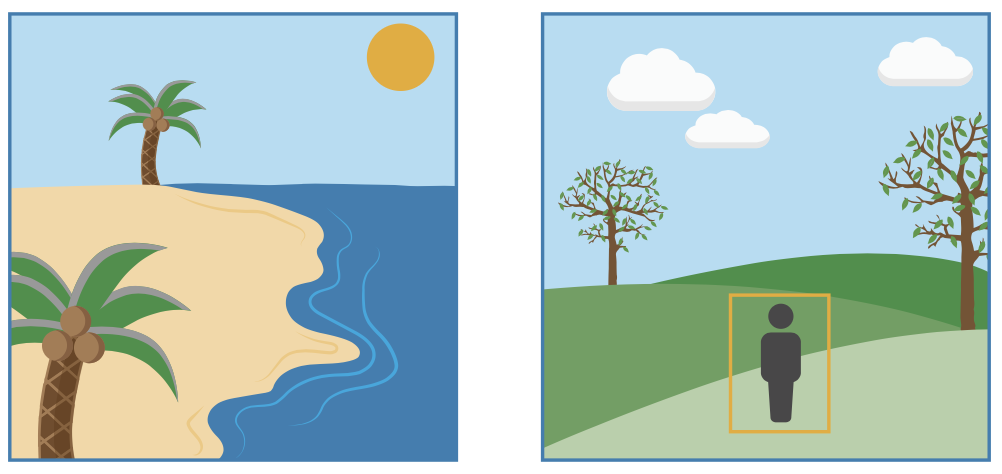
\includegraphics[scale=0.45]{objectdetectie.png}
\end{center}


\subsection{Werking van objectherkenning}
Om objectherkenning toe te passen kan je gebruik maken van twee verschillende manieren, namelijk 'Machine Learning' en 'Deep learning'. Beide technieken zullen objecten gaan herkennen, maar ze zijn verschillend op vlak van uitvoering.

\subsubsection{Machine learing}
Machine learning maakt gebruik van classificatie om een bepaald object te herkennen. Ten eerste zal men een trainingset opstellen, dit gebeurt door een verzameling van afbeeldingen samen te stellen en vervolgens de relevante punten aan te duiden. Het is zeer belangrijk om de juiste relevante punten aan te duiden, anders zal het systeem verkeerd getraind worden, waardoor men vervolgens een verkeerde output zal verkrijgen. Deze punten zullen er voor zorgen dat het systeem verschillende categorieën herkent. Vervolgens zal het leermodel deze informatie gebruiken om nieuwe objecten (objecten die nog niet gekend zijn in de trainingset) te analyseren en te classificeren.

\begin{center}
	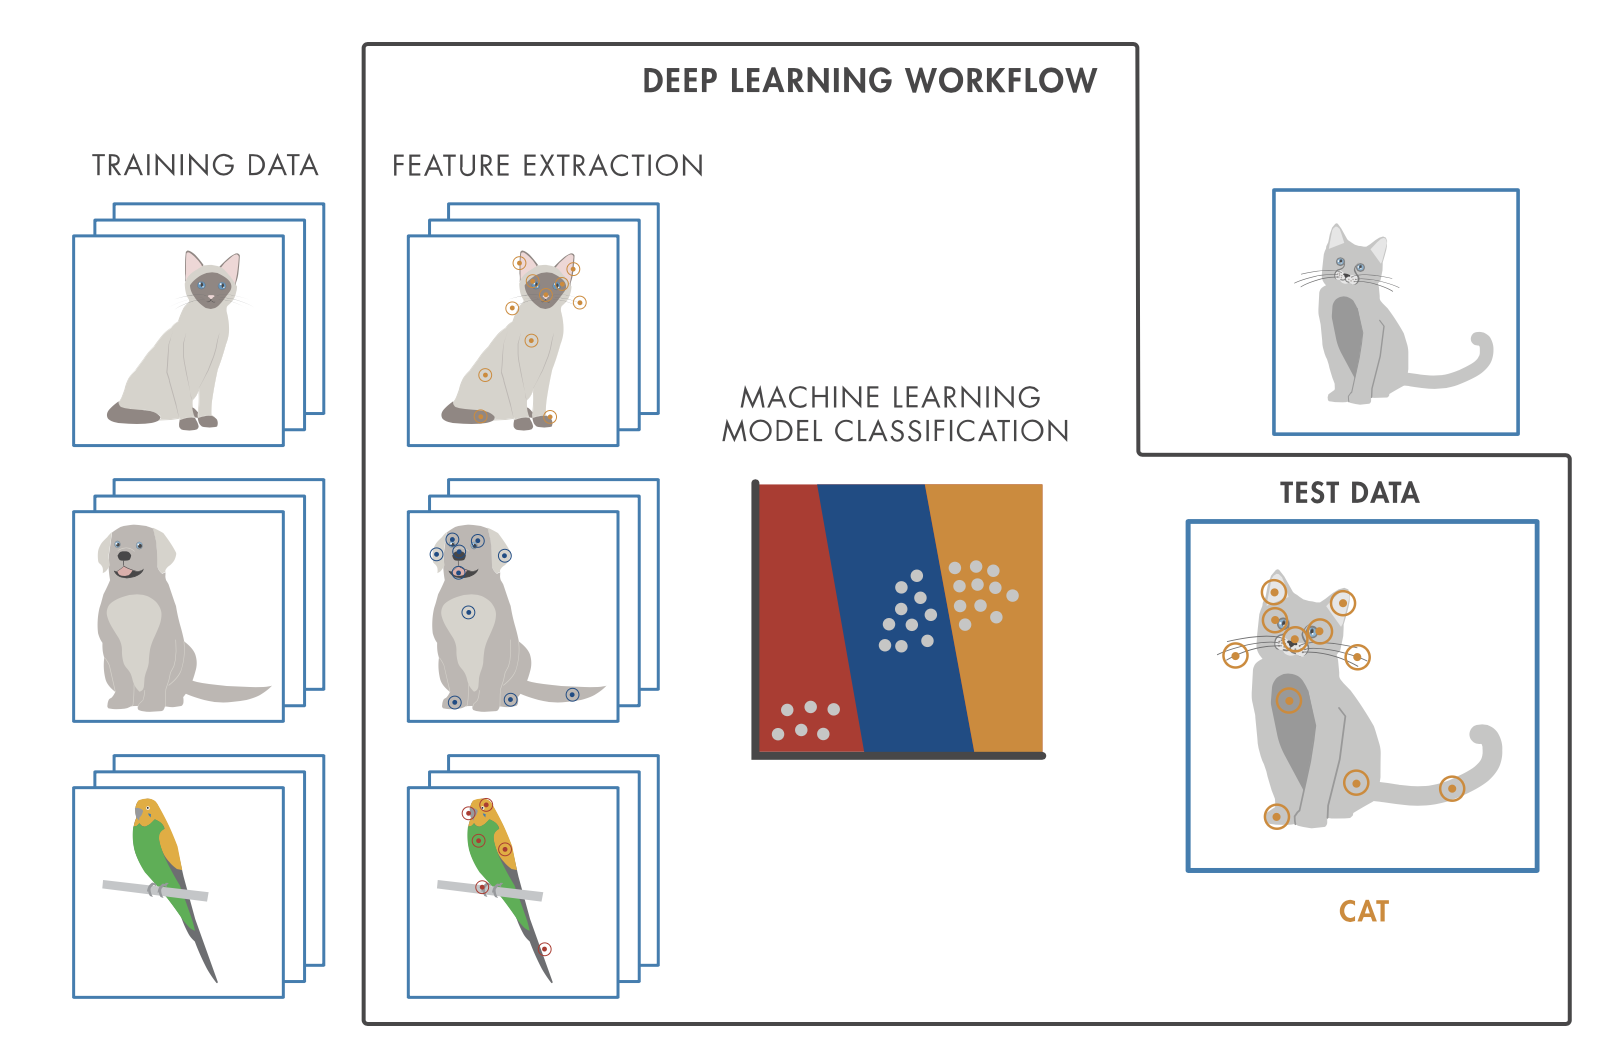
\includegraphics[scale=0.4]{machinelearning.png}
\end{center}

\subsubsection{Deep learning}
Deep learning maakt gebruik van convulationele neurale netwerken (CNN) om objecten te herkennen. Een CNN kan automatisch de aanhangende kenmerken van een object leren om dat object te identificeren, dit betekent dat een CNN bijvoorbeeld het verschil tussen auto's en vrachtwagens kan herkennen door middel van duizenden afbeeldingen te analyseren en vervolgens te leren welke kenmerken juist verschillend zijn.

\begin{center}
	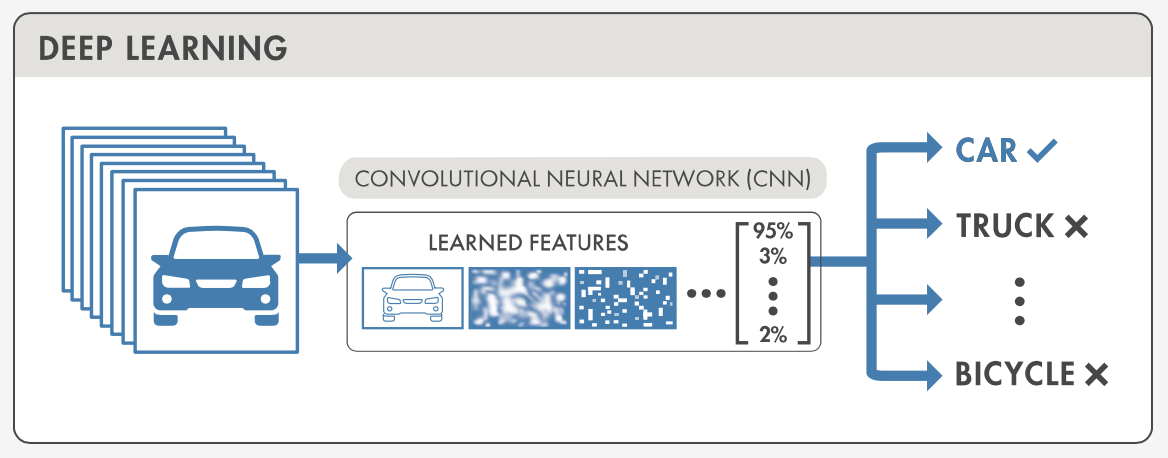
\includegraphics[scale=0.47]{deeplearning.png}
\end{center}

\section{AR (Augmented reality)}
Het concept AR is vandaag de dag niet meer uit het straatbeeld weg te denken, het wordt bijvoorbeeld gebruikt bij de Instagram -en Snapchat filters. Augmented reality of AR is een interactieve ervaring met de omgeving waarin objecten die zich in de echte wereld bevinden worden versterkt door computergegenereerde objecten. AR is iets wat al even bestaat, het werd bijvoorbeeld al gebruikt bij één van de eerste straaljagers, het visier van de piloot wordt in dit voorbeeld ondersteund door een computergegenereerd object dat de vijand zou moeten lokaliseren. Augmented reality werd pas populair bij de modale mens wanneer Naintic Pokemon Go lanceerde, het werd één van de meest gekende smarthonegames. In 2017 introduceerde Android en Apple, AR Core en AR Kit, het werd vervolgens voor developers veel eenvoudiger om AR-applicaties te creëren.

Het doel van Augemented reality in deze bachelorproef is om de route op een zo efficiënt mogelijke manier aan te geven, dit betekent dat er geen pijlen door objecten mogen gaan. Om een beeld te kunnen scheppen over het effectieve doeleinde, heeft men alvast een voorbeeldfoto toegevoegd.

\begin{center}
	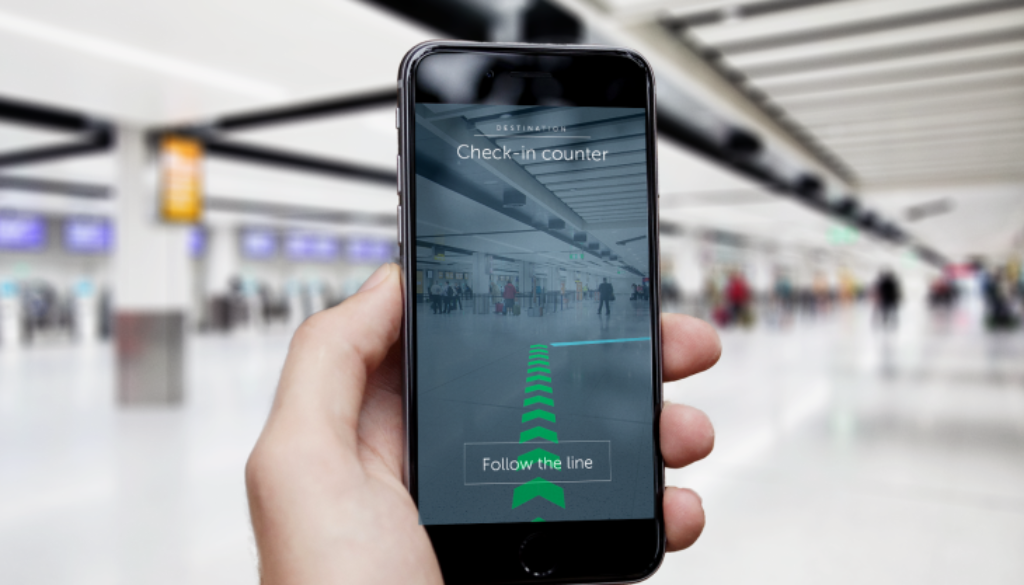
\includegraphics[scale=0.25]{wayfinding.png}
\end{center}

\subsection{Werking van Augmented realtiy}
Augmented reality kan momenteel op drie verschillende manieren worden uitgewerkt, namelijk door middel van SLAM, herkenning gebaseerd en locatie gebaseerd.

\subsubsection{SLAM (Simultaneous Localization and Mapping)}
Simultaneous Localization and Mapping of SLAM is de manier die het meest effectief en efficiënt werkt. SLAM lokaliseert sensoren ten opzichte van hun omgeving en brengt tegelijkertijd de omgeving in kaart, het is dus een zeer goede aanpak om complexe AR-simulatieproblemen op te lossen. Het SLAM-systeem is in feite een set van algoritmen die gericht zijn op het oplossen van gelijktijdige lokalisatie en het in kaart brengen van problemen. De meeste Augmented realitykits zijn reeds uitgerust met de mogelijkheid tot een SLAM-aanpak.

\subsubsection{Herkenning gebaseerd}
Herkenning gebaseerd gebruikt de camera van het gebruikte apparaat om bepaalde visuele markers of objecten te identificeren. Deze AR-technologie is bijgevolg zeer afhankelijk van de kwaliteit van de gebruikte camera, als deze de markers niet goed kan identificeren, dan zal het AR mechanisme niet goed werken.

Bij deze manier is het ook mogelijk om de positie en oriëntatie te berekenen. De markers op het scherm worden vervangen door een overeenkomstig 3D-object, dit maakt het mogelijk om het object meer in detail te bekijken door het bijvoorbeeld te roteren zodat men meerdere invalshoeken kan observeren.

\subsubsection{Locatie gebaseerd}
Locatie gebaseerd of 'markerless augmented reality' is een AR-technologie die alleen gebruikt maakt van een GPS, digitaal kompas, snelheidsmeter of versnellingsmeter om gegevens over de locatie te verzamelen, de augmented reality visualisaties worden met behulp van deze informatie geactiveerd. Een smartphone heeft genoeg sensoren om deze manier te kunnen realiseren. 

\section{AI + AR}
De samenhang van Artificiële intelligentie en Augmented reality is zeer cruciaal bij het optimaliseren van een wayfinding applicatie. Ten eerste is het belangrijk dat de objecten op een correcte manier worden herkend. Ten tweede is het zeer belangrijk dat de bevindingen van de objectherkenning op een correcte manier worden vertaald naar de AR omgeving. 


